\setlength{\columnsep}{3pt}
\begin{flushleft}

	In case of \textbf{primitive type arrays}, as array elements, you can provide any type which can be \textbf{implicitly promoted to declared type}.
	\begin{figure}[h!]
		\centering
		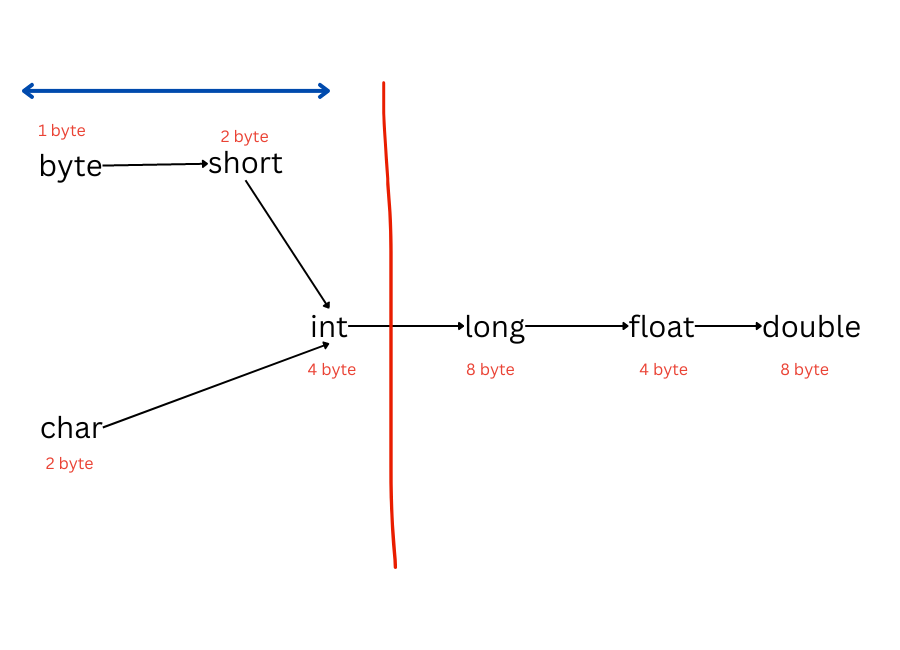
\includegraphics[scale=.4]{content/chapter4/images/allow.png}
	\end{figure}	
	Example:
	\codeblock{
		int[] x = new int[5]; \\
		x[0] = 10; \\
		x[1] = 'a'; \\
		byte b = 20; \\
		x[2] = b; \\
		short s = 30; \\
		x[3] = s; \\
		x[4] = 10L; \xmark
	}
	
	Similary, in case of float type arrays, the allowed datatypes are:
	\begin{itemize}
		\item byte
		\item short
		\item char
		\item int
		\item long
		\item float
	\end{itemize}
		
\end{flushleft}
